%%%%%%%%%%%%%%%%%%%%%%%%%%%%%%%%%%%%%%%%%%%%%%%%%%%%%%%%%%%%%%%%%
% Dissertacao de Mestrado / Dept Fisica, CFM, UFSC              %
% Lacerda@UFSC - 2013                                           %
%%%%%%%%%%%%%%%%%%%%%%%%%%%%%%%%%%%%%%%%%%%%%%%%%%%%%%%%%%%%%%%%%

%:::::::::::::::::::::::::::::::::::::::::::::::::::::::::::::::%
%                                                               %
%                          Capítulo 2                           %
%                                                               %
%:::::::::::::::::::::::::::::::::::::::::::::::::::::::::::::::%

%***************************************************************%
%                                                               %
%                      CALIFA & PyCASSO                         %
%                                                               %
%***************************************************************%

\chapter{O projeto CALIFA e o {\em pipeline} PyCASSO}
\label{sec:CALePyC}

As observações do universo modificaram completamente o nosso modo de viver,
pensar, compreender-se. Aprendemos a contar os dias, desenvolvemos um sistema
de meses, estações do ano, movimentos das marés, entre outras coisas que já são
parte do senso comum, mas que um dia foram o estado da arte da ciência. É assim
que surge o CALIFA: um projeto que está modificando nossa maneira de ver e
pensar as galáxias no nosso universo de forma que entendamos melhor a nossa também.

Com a massiva quantidade de dados obtidos, resultado direto de um projeto de
ciência de ponta, vem também a dificuldade da interpretação dos dados. No caso
do CALIFA, através da {\em pipeline} PyCASSO \citep{CidFernandes2013a}, a
programação investigativa se torna simples e ao mesmo tempo robusta,
facilitando a construção de todo tipo de resultados, sejam eles \ojo matemáticos
ou físicos.

%***************************************************************%
%                                                               %
%                            CALIFA                             %
%                                                               %
%***************************************************************%

\section{O survey CALIFA}
\label{sec:CALePyC:Apresent}

No sul da Espanha, mais precisamente em {\em Sierra de Los Filabres}
(Andalucía), está situado o germano-espânico {\em Calar Alto Observatory}. O
projeto CALIFA está sendo possível através de observações de o maior de seus
$3$ telescópios ($3.5$m) e terá ao todo $\sim 600$ objetos ao longo de $250$
noites de observação. Em comparação com o \SDSS, o CALIFA terá a mesma ordem de
número de espectros para estudo ($\sim10^6$), mas, apesar de um número menor de
galáxias, graças ao IFU será o com melhor completeza por objeto. Existem alguns poucos
surveys IFU e todos com, além de poucos objetos e FoV menor, focos de estudo
muito estreitos, dificultando o legado do survey para outras pequisas
científicas mais abrangentes \citep[SAURON; ][região central de 72 galáxias
com $z < 0.01$.]{de-Zeeuw2002} \citep[PINGS; ][algumas galáxias muito próximas
($\sim 10$ Mpc) e o estudo atual de 70 (U)LIRGs com $z <0.26$]{RosalesOrtega2010}
\citep[VENGA; ][$30$ galáxias espirais]{Blanc2010}. Apesar de ser primariamente
construído para o estudo da física bariônica da evolução de galáxias, o CALIFA
está projetado para que seu legado seja bem abrangente, possibilitando diversos
tipos de estudos em diversas áreas. Outros surveys IFU ainda estão por vir, como
SAMI \citep{Croom2012} e MaNGA \citetext{Bundy et al., in prep}. 

\subsection{A ``{\em colméia}'' de fibras - os dados do CALIFA que usamos neste
trabalho}

A amostra mãe do projeto comporta $939$ galáxias com {\em redshifts} entre
$0.005 < z < 0.03$ que distribuídas cobrem o diagrama cor-magnitude com $M_r <
-18$ (Figura \ref{fig:cm-uzMz}) em uma ampla variedade de tipos morfologicos,
massa em estrelas, condições do gás ionizante. Para melhor aproveitar o {\em
FoV} ({\em field-of-view}\footnote{campo de visão}) do instrumento de IFU é
feito também um corte em dimensão ($\sim1'$ em diâmetro). No telescópio usado
para o projeto está instalado o equipamento Potsdam Multi Aperture Spectrograph
\citep[PMAS; ][]{Roth2005} no modo PPAK \citep{Verheijen2004, Kelz2006}
formando um espectrofotômetro de campo integrado com um {\em bundle} de $382$
fibras (Figura \ref{fig:BundlePPAK}), das quais, $331$ são para observação dos
objetos, outras $36$ para \ojo \textcolor{blue}{\em sky background sample} e
outras $15$ para calibração. As {\em science fibers} ($331$) cobrem um campo de
visão hexagonal de $74"$ x $64"$ que, através de uma técnica de três pontos de
dithering \ojo torna possível a observação de $100\%$ do campo.

\begin{figure}
    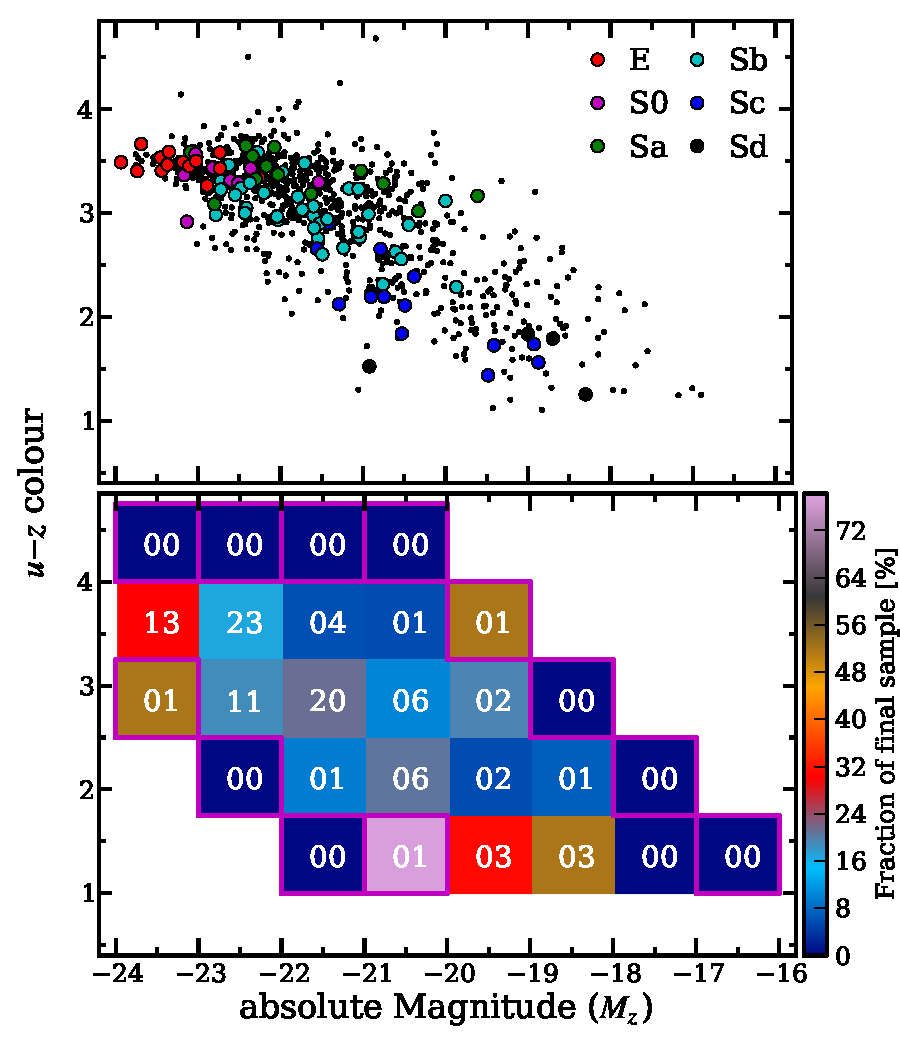
\includegraphics[height=0.5\textwidth]{figuras/figHusemann2013Fig2.pdf}
    \caption[Diagrama cor-magnitude para as galáxias do CALIFA.]
    {Distribui\c{c}\~ao das galáxias do CALIFA no diagrama $u-z$ vs. $M_z$. 
    {\em Painel superior}: Em pontos pretos est\~ao as galáxias pertencente a
    amostra-m\~ae e em cores as galáxias presente no CALIFA DR1. As diferentes
    cores representam os diferentes tipos morfológicos. {\em Painel inferor}: A
    fra\c{c}\~ao de galáxias observadas pelo DR1 em rela\c{c}\~ao a
    amostra-m\~ae. Retirado de \citet{Husemann2013}, figura $2$.}
    \label{fig:cm-uzMz}
\end{figure}

Os dados são reduzidos utilizando o programa CALIFA Pipeline versão 1.3c,
descrito em \citet{Husemann2013}. Os espectros vêm em duas configurações: a
V$500$ cobrindo de $\sim3700$ até $7000$ \AA\ com resolução de $\sim6$ \AA\ 
de largura à meia altura (FWHM) e a V$1200$ ($\sim3650-4600$ \AA\  FWHM
$\sim2.3$ \AA). A cobertura do V$500$ sería ideal para os propósitos de ciência feita pelo
\starlight mas por problemas com {\em vignetting} com a parte azul dessa
configuração, os dados são reamostrados numa combinação das duas, criando uma
que chamamos de COMBO. A parte com $\lambda < 4600$ \AA\  vem do V$1200$ e a
outra parte do V$500$. Os espectros foram reamostrados no mesmo FWHM do V$500$.

\begin{figure}
    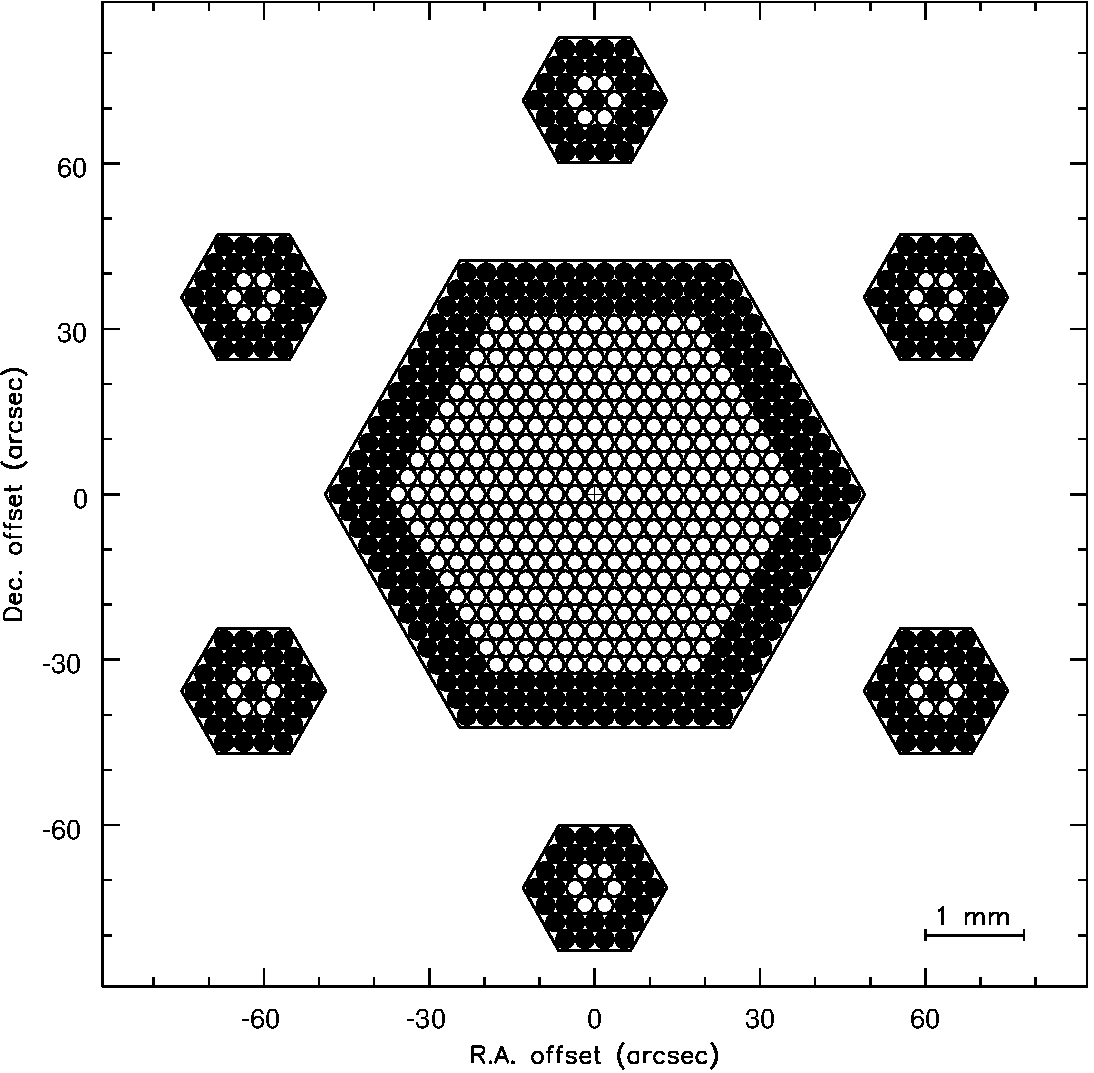
\includegraphics[height=0.5\textwidth]{figuras/figVerheijen2004Fig5.pdf}
    \caption[Configura\c{c}\~ao do {\em bundle} de fibras do PPMAS/PPAK.]
    {Este é o esquema com o {\em bundle} hexagonal com as 331 fibras de
    observação e mais 36 de amostra de céu. Retirado de \citet{Verheijen2004},
    figura $5$.}
    \label{fig:BundlePPAK}
\end{figure}

Após os dados passarem pelo CALIFA {\em Pipeline} v$1.3$c, os parâmetros físicos
aqui usados vêm do PyCASSO que organiza as saídas da síntese de populações
estelares resultantes da execução de cada espectro do IFU pelo \starlight
\citep{CidFernandes2005} como descrito em \citet{CidFernandes2013a} e também na
próxima seção.

%***************************************************************%
%                                                               %
%                            PyCASSO                            %
%                                                               %
%***************************************************************%

\section{O {\em pipeline} PyCASSO}
\label{sec:CALePyC:PyCASSO}

% End of this chapter
